%ps1.tex
%notes for the course Probability and Statistics COMS10011 
%taught at the University of Bristol
%2018_19 Conor Houghton conor.houghton@bristol.ac.uk

%To the extent possible under law, the author has dedicated all copyright 
%and related and neighboring rights to these notes to the public domain 
%worldwide. These notes are distributed without any warranty. 

\documentclass[11pt,a4paper]{scrartcl}
\typearea{12}
\usepackage{graphicx}
%\usepackage{pstricks}
\usepackage{listings}
\usepackage{color}
\lstset{language=C}
\usepackage{fancyhdr}
\pagestyle{fancy}
\lfoot{\texttt{github.com/COMS10011/2018\_19}}
\lhead{COMS10007 ps1 - Conor}
\begin{document}

\section*{Problem Sheet 1}

\begin{center}
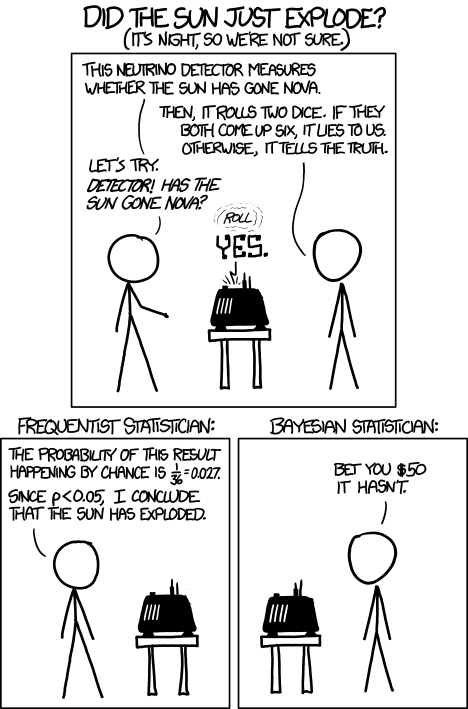
\includegraphics[width=7.5cm]{frequentists_vs_bayesians.png}
\end{center}

This is an xkcd cartoon that someone posted to the unit reddit, it is
\texttt{https://xkcd.com/1132/}. It is also worth reading Randall Monroe's comment on the response to this cartoon:

\begin{quote}
Hey! I was kinda blindsided by the response to this comic.

I�m in the middle of reading a series of books about forecasting
errors (including Nate Silver�s book, which I really enjoyed), and
again and again kept hitting examples of mistakes caused by blind
application of the textbook confidence interval approach.

Someone asked me to explain it in simple terms, but I realized that in
the common examples used to illustrate this sort of error, like the
cancer screening/drug test false positive ones, the correct result is
surprising or unintuitive. So I came up with the sun-explosion
example, to illustrate a case where na�ve application of that
significance test can give a result that�s obviously nonsense.

I seem to have stepped on a hornet�s nest, though, by adding
�Frequentist� and �Bayesian� titles to the panels. This came as a
surprise to me, in part because I actually added them as an
afterthought, along with the final punchline. (I originally had the
guy on the right making some other cross-panel comment, but I thought
the �bet� thing was cuter.)

The truth is, I genuinely didn�t realize Frequentists and Bayesians
were actual camps of people�all of whom are now emailing me. I thought
they were loosely-applied labels�perhaps just labels appropriated by
the books I had happened to read recently�for the standard textbook
approach we learned in science class versus an approach which more
carefully incorporates the ideas of prior probabilities.

I meant this as a jab at the kind of shoddy misapplications of
statistics I keep running into in things like cancer screening (which
is an emotionally wrenching subject full of poorly-applied
probability) and political forecasting. I wasn�t intending to
characterize the merits of the two sides of what turns out to be a
much more involved and ongoing academic debate than I realized.

A sincere thank you for the gentle corrections; I�ve taken them to
heart, and you can be confident I will avoid such mischaracterizations
in the future!

At least, 95.45\% confident.
\end{quote}
Thanks again to the person who posted this.

\subsection*{Useful facts}

\begin{itemize}

\item \textbf{Combinations} The number of ways of choosing $r$ items out of $n$ is 
\begin{equation}
\left(\begin{array}{c}n\\r\end{array}\right)=\frac{n(n-1)(n-2)\ldots(n-r+1)}{r(r-1)(r-2)\ldots 1}=\frac{n!}{r!(n-r)!} 
\end{equation}

\item \textbf{Bayes's rule}
\begin{equation}
P(A|B)=\frac{P(B|A)P(A)}{P(B)}
\end{equation}

\item \textbf{Set notation}: If $C$ is a subset, the complement of $C$, that is the set of all the elements not in $C$, is written $\bar{C}$. For an event $C$, $\bar{C}$ is the event of $C$ not happening.
 
\item \textbf{Cards}: 52 cards made up of four suits; in each suit
  there are 13 values, ace, two through to ten and the jack, queen,
  kind.

\item \textbf{Poker hands}: the number of poker hands is 
\begin{equation}
\left(\begin{array}{c}52\\5\end{array}\right)= 2598960
\end{equation}

\end{itemize}

\newpage

\subsection*{Questions}

Four questions, each worth two marks with two marks for attendance.

\begin{enumerate}



\item In the poker hand \textsl{two pair} there are two pairs of cards
  with each card in the pair matched by value; the fifth card has a
  different value to either pair. What is the probability of two pairs
  when five cards are drawn randomly. In a \textsl{full house} there is one
  pair and one triple, what is the probability of getting a full
  house?

\item A student answers a multiple choice question with four options,
  one of which is correct. 80\% of students know the answer, 20\% of
  students guess and choose randomly. If a student gets the answer
  correct what is the chance they knew the answer.

\item In the xkcd cartoon above, what is the chance the Bayesian will
  win his or her bet if the chance the sun has exploded is one in a
  million? In reality the chance is, of course, much less than one in
  a million! Show the answer to six decimal places.

\item A three-sided dice is rolled three times. $X$ is the sum of the
  largest two values. Write down the probability distribution for $X$.

\end{enumerate}

\end{document}

